\chapter{Analisis Dan Rancangan Prototipe Aplikasi Pencegah Distraksi}

Bab 3 Analisis dan Rancangan Aplikasi Pencegah Distraksi berisi tentang identifikasi permasalahan, hingga penjelasan solusi prototipe aplikasi yang menjadi dasar dari tugas akhir ini. Setelah melakukan studi literatur pada Bab II, maka tahap selanjutnya dilakukan sesuai dengan metodologi yang telah ditetapkan yaitu pendekatan \textit{user-centered design} (UCD) menurut ISO 9241-210.

\section{Analisis Permasalahan}
\label{sec:analisis_masalah}

Penggunaan \textit{smartphone} sudah menjadi bagian dari kehidupan sehari-hari manusia, tapi penggunaan dengan kadar yang tidak memunculkan pengaruh buruk pada kesehatan mental penggunanya. Menurut \textcite{10.1371/journal.pone.0083558}, adiksi terhadap \textit{smartphone} belum terdaftar sebagai \textit{behavourial addiction} dalama DSM-5 (Diagnostic and Statistical Manual of Mental Disorders), namun korban adiksi \textit{smartphone} telah menunjukkan tingkat adiksi yang sama dengan korban adiksi narkotika dan alkohol. Korban adiksi \textit{smartphone} mengalami permasalahan pada kesehatan mental dan interaksi sosialnya yang dapat terlihat dari kualitas interaksi sesama manusia secara langsung. \parencite{Roffarello2019} \textit{Smartphone} juga berperan sebagai sumber distraksi yang mengalihkan perhatian korban adiksi dari kegiatan yang penting. Distraksi tersebut dapat berupa notifikasi yang muncul pada \textit{smartphone}, atau keinginan pengguna untuk menggunakan \textit{smartphone}. Pengguna dengan adiksi \textit{smartphone} dilaporkan mengalami penurunan produktivitas dan stress.

% Produktivitas yang rendah dapat memengaruhi perkembangan bisnis dan kesehatan mental

Dalam upaya mengatasi adiksi \textit{smartphone}, Google meluncurkan sebuah langkah Digital Wellbeing dalam konferensi Google I/O pada tahun 2018. Digital Wellbeing adalah sebuah filosofi desain yang akan diterapkan pada produk-produk Google dengan tujuan untuk membangun hubungan yang lebih baik antara pengguna dengan teknologi yang digunakan. Konsep dari Digital Wellbeing mengajak pengguna produk Google untuk mengambil kendali teknologi agar dapat memberikan manfaat dan potensial semaksimal mungkin serta membantu untuk mencapai tujuan yang diinginkan, melainkan menjadi pengganggu, distraksi, atau rintangan. \parencite{google2019dwcourse} Pada konferensi tersebut, Google juga meluncurkan aplikasi dengan nama yang sama sebagai wujud nyata dari langkah Digital Wellbeing, dan sejak versi Android 10 aplikasi ini sudah terintegrasi pada sistem operasi buatan Google, Android.

Keputusan Google untuk mengintegrasikan aplikasi ke dalam sistem operasi Android memunculkan banyak opini. Berdasarkan review aplikasi pada Google Play Store, banyak reviewer melaporkan ketidakpuasan atas keputusan Google untuk menghilangkan kemampuan untuk meng-\textit{uninstall} aplikasi, mengakibatkan turunnya performa \textit{smartphone} pengguna, serta mengambil tempat penyimpanan \textit{smartphone} yang seharusnya dapat dimanfaatkan untuk hal lain, sehingga pengguna dapat menganggap aplikasi Digital Wellbeing sebagai sebuah bloatware. Bloatware adalah sebuah software yang tidak diinginkan yang dapat memperlambat kinerja suatu perangkat dan biasanya sudah dipasang pada perangkat dari pabrik, baik oleh perusahaan manufaktur perangkat atau penyedia layanan yang bekerja sama dengan perusahaan tersebut. \parencite{nordvpn2021bloatware} Namun Google tetap memberikan pengaturan pada aplikasi untuk tidak melakukan pemantauan, dan sebagai pengaturan bawaan fitur-fitur dari Digital Wellbeing selain pemantauan aktivitas tidak diaktifkan.

Aplikasi Digital Wellbeing milik Google tidak luput dari berbagai permasalahan dari sisi desain interaksi. Padahal masalah yang sering ditemukan dari aplikasi bawaan \textit{smartphone} yang membuatnya bisa disebut sebagai bloatware adalah terbatasnya fungsionalitas dari aplikasi tersebut. \parencite{forbes2018bloatware} Alasan ini beserta kekurangan yang ditemukan dari aplikasi berdasarkan hasil analisis akan digunakan sebagai pendukung solusi dari tugas akhir ini. Setelah melakukan analisis terhadap data ulasan aplikasi Digital Wellbeing yang diperoleh melalui Google Play Store, berikut adalah daftar masalah yang ingin diselesaikan dalam pengerjaan tugas akhir.

% Tetapi,  hal   Selain itu da membuat aplikasi Digital Wellbeing tersembunyi dari \textit{app library}, serta    
% \textit{smartphone}-nya. Salah satu fungsionalitas dari aplikasi adalah melakukan pemantauan terhadap penggunaan aplikasi dan \textit{smartphone}. 

% membatasi akses pengguna terhadap aplikasi, serta memberikan pengingat atas jumlah penggunaan yang tinggi. 

% Sejak sistem operasi Android versi Android 10, Google telah mengintegrasikan aplikasi Digital Wellbeing sebagai bagian dari langkah Google dalam menerapkan konsep Digital Wellbeing. \parencite{google2021dwsupport} Keputusan Google untuk mengintegrasi aplikasi ini berarti pengguna \textit{smartphone} Android tidak secara sadar menginstallnya. Sebagai aplikasi yang sudah terintegrasi, memunculkan kemungkinan aplikasi tersebut dapat memperlambat performa dari \textit{smartphone} atau mengambil tempat penyimpanan \textit{smartphone} yang seharusnya dapat dimanfaatkan untuk hal lain. Namun, fitur    

% Sebagaimana yang telah dibahas pada subbab \ref{sec:latarbelakang}, aplikasi Digital Wellbeing yang terdapat pada smartphone berbasis Android memiliki beberapa masalah pada desain interaksinya. Pada dasarnya, inti masalah dari desain interaksi aplikasi Digital Wellbeing adalah kurang efektif dalam menghambat pengguna mengakses aplikasi-aplikasi yang menurunkan tingkat produktivitas pengguna, serta kurang efektif dalam mempromosikan kebiasaan-kebiasaan yang lebih baik dalam penggunaan gawai dalam kehidupan sehari-hari. Daftar permasalahan desain interaksi yang terdapat pada aplikasi Digital Wellbeing dicantumkan pada Tabel \ref{tab:daftar_permasalahan}. Rincian mengenai permasalahan dapat dilihat pada Lampiran \ref{chpt:rincian_analisis_permasalahan}.

\begin{table}[ht]
  \centering
  \fontsize{10}{12}
  \caption{Daftar Permasalahan}
  \label{tab:daftar_permasalahan}
  \vspace{0.2cm}
  \begin{tabular}{|p{0.12\textwidth}|p{0.81\textwidth}|}
  \hline
  ID    & Masalah Aplikasi Digital Wellbeing \\ \hline
  M-01    & Fitur-fitur pada aplikasi Digital Wellbeing kurang dapat membatasi akses pengguna dengan cukup ketat \\ \hline
  M-02    & Fitur-fitur pada aplikasi Digital Wellbeing kurang memberikan fleksibilitas dalam menunda pembatasan akses pengguna \\ \hline
  M-03    & Aplikasi Digital Wellbeing kurang memberikan fleksibilitas bagi pengguna dalam mengatur jadwal aktivasi fitur \\ \hline
  M-04    & Aplikasi Digital Wellbeing tidak dapat mengelompokkan aplikasi berdasarkan kategori yang ditentukan oleh pengguna \\ \hline
  M-05    & Aplikasi Digital Wellbeing kurang memberikan laporan yang komprehensif tentang aktivitas pengguna \textit{smartphone} \\ \hline
  % M-06    & Aplikasi Digital Wellbeing saat ini hanya memiliki 1 buah \textit{widget} yang dapat menampilkan total \textit{screentime} pengguna \textit{smartphone} dan 3 aplikasi dengan penggunaan tertinggi di hari tersebut\\ \hline
  \end{tabular}
\end{table}

Sebagai batasan masalah, perlu disebutkan bahwa tidak adanya kemampuan untuk menghapus aplikasi Digital Wellbeing dari perangkat tidak akan dijadikan rumusan masalah, hal ini memiliki alasan yaitu menghapus aplikasi dari perangkat bukanlah solusi yang sejajar dengan masalah yang ingin diselesaikan dari konsep Digital Wellbeing. Selain itu, masalah yang berhubungan dengan performa aplikasi atau dampaknya pada perangkat tidak akan dijadikan rumusan masalah, namun saat pembangunan solusi hal ini akan diperhatikan agar tidak mengganggu tahap pengujian.


\section{Analisis Solusi}
\label{sec:analisis_solusi}

% Dari permasalahan yang telah diuraikan pada subbab \ref{sec:analisis_masalah}, terdapat beberapa solusi yang dapat diimplementasikan ke dalam aplikasi pencegah distraksi untuk mencapai tujuan dari aplikasi Digital Wellbeing dengan lebih baik yaitu menghambat akses pengguna terhadap aplikasi distraksi secara efektif dan memotivasi pengguna untuk mengubah pola penggunaan aplikasi secara general. Setiap solusi akan dijelaskan tentang permasalahan apa yang akan diselesaikan. Solusi yang ditawarkan untuk menyelesaikan masalah yang telah dianalisis dicantumkan pada Tabel \ref{tab:daftar_solusi}. Rincian mengenai solusi tersebut dapat dilihat pada Lampiran \ref{chpt:rincian_analisis_solusi}.

Berdasarkan hasil analisis permasalahan yang dilakukan, maka solusi yang akan dibuat adalah sebuah prototipe aplikasi pencegah distraksi dengan tampilan mendekati aplikasi Digital Wellbeing yang dapat menyelesaikan rumusan masalah yang telah disebutkan pada Tabel \ref{tab:daftar_permasalahan}. Pada Tabel \ref{tab:daftar_solusi} terdapat pemetaan rumusan masalah kepada rancangan solusi dalam bentuk kebutuhan fungsional dan kebutuhan interaksi yang akan dimiliki oleh prototipe aplikasi

% \singlespacing
% >{\setlength{\baselineskip}{0.75\baselineskip}}p{0.17\linewidth}
\begin{longtable}[c]{|p{0.07\textwidth}|p{0.3\textwidth}|p{0.4\textwidth}|p{0.1\textwidth}|}
  % \centering
  % \fontsize{10}{12}
  \caption{Daftar Solusi}
  \label{tab:daftar_solusi} \\

  \hline
  ID  & Kebutuhan Fungsional & Kebutuhan Interaksi & Kode Masalah \\ \hline \endhead

  \hline \endfoot

  S-01
  & \multirow{2}{0.3\textwidth}{Prototipe aplikasi dapat membatasi akses pengguna dengan cukup ketat}
  & Pengguna dapat memanfaatkan fitur "Take a break" pada Focus Mode hanya sebanyak waktu yang ditentukan per harinya
  & \multirow{4}{0.1\textwidth}{M-01} \\ \cline{1-1} \cline{3-3}
  
  S-02 &  
  & Pengguna perlu membuka kunci saat melakukan pengaturan pada fitur Focus Mode
  & \\ \cline{1-1} \cline{3-3}
  
  S-03 &  
  & Pengguna dapat memilih untuk menghilangkan kemampuan mematikan Focus Mode selama fitur berjalan
  & \\ \cline{1-1} \cline{3-3}
  
  S-04 &  
  & Pengguna perlu membuka kunci saat melakukan pengaturan pada fitur App Timer
  & \\ \cline{1-1} \cline{3-3}
  
  S-05 &  
  & Pengguna dapat membatasi aplikasi yang dapat diakses saat menggunakan fitur Bedtime Mode
  & \\ \cline{1-1} \cline{3-3}
  
  S-06 &  
  & Pengguna dapat menunda fitur Bedtime Mode hanya sebanyak waktu yang ditentukan per harinya
  
  & \\ \hline
  % ===========================
  S-07
  & \multirow{3}{0.3\textwidth}{Prototipe aplikasi dapat memberikan fleksibilitas dalam menunda pembatasan akses pengguna}
  & Pengguna dapat diingatkan terhadap batas App Timer beberapa saat lebih lama
  & \multirow{2}{0.1\textwidth}{M-02} \\ \cline{1-1} \cline{3-3}
  
  S-08 &  
  & Pengguna dapat diberikan tampilan durasi penggunaan aplikasi yang terdaftar dalam App Timer pada \textit{notification bar}
  & \\ \cline{1-1} \cline{3-3}
  
  S-09 &  
  & Pengguna dapat mengambil waktu tambahan yang terbatas untuk menggunakan aplikasi yang terdaftar dalam App Timer
  
  & \\ \hline
  % ===========================
  S-10
  & \multirow{2}{0.3\textwidth}{Prototipe dapat memberikan fleksibilitas bagi
  pengguna dalam mengatur jadwal aktivasi fitur}
  & Pengguna dapat membuat lebih dari 1 jadwal per minggu untuk fitur Focus Mode
  & \multirow{4}{0.1\textwidth}{M-03} \\ \cline{1-1} \cline{3-3}
  
  S-11 &  
  & Pengguna dapat menentukan waktu istirahat pada saat membuat jadwal untuk fitur Focus Mode
  & \\ \cline{1-1} \cline{3-3}
  
  S-12 &  
  & Pengguna dapat memilih membuat jadwal untuk membuka akses atau membatasi akses terhadap aplikasi untuk fitur Focus Mode   
  & \\ \cline{1-1} \cline{3-3}
  
  S-13 &  
  & Pengguna dapat mengatur waktu akhir hari untuk App Timer dan pelacakan data penggunaan harian  
  & \\ \cline{1-1} \cline{3-3}
  
  S-14 &  
  & Pengguna dapat membuat lebih dari 1 jadwal per minggu untuk fitur App Timer   
  & \\ \cline{1-1} \cline{3-3}
  
  S-15 &  
  & Pengguna dapat memilih membuat jadwal untuk membuka akses atau membatasi akses terhadap aplikasi untuk fitur App Timer   
  & \\ \cline{1-1} \cline{3-3}
  
  S-16 &  
  & Pengguna dapat membuat jadwal batas penggunaan per minggu untuk fitur App Timer   
  % & \\ \cline{1-1} \cline{3-3}

  & \\ \hline
  % ===========================
  S-17
  & Prototipe aplikasi dapat mengelompokkan aplikasi berdasarkan kategori yang ditentukan oleh pengguna
  & Pengguna dapat mengelompokkan aplikasi berdasarkan kategori yang ditentukan pengguna
  & M-04 \\ \hline
  
  % ===========================
  S-18
  & \multirow{3}{0.3\textwidth}{Prototipe aplikasi dapat memberikan laporan yang komprehensif tentang aktivitas pengguna smartphone}
  & Pengguna dapat melihat data waktu Focus Mode yang ditempuh
  & \multirow{2}{0.1\textwidth}{M-05} \\ \cline{1-1} \cline{3-3}

  S-19 &  
  & Pengguna dapat melihat laporan data rata-rata penggunaan \textit{smartphone} harian per minggu 
  & \\ \cline{1-1} \cline{3-3}

  S-20 &  
  & Pengguna dapat melihat laporan data rata-rata penggunaan aplikasi harian per minggu 
  & \\ \cline{1-1} \cline{3-3}

  S-21 &  
  & Pengguna dapat melihat laporan aktivitas lebih dari 10 hari yang lalu
  & \\ \cline{1-1} \cline{3-3}

  S-22 &  
  & Pengguna dapat melihat laporan aktivitas dengan periode waktu per bulan dan per tahun 
  & \\ \cline{1-1} \cline{3-3}

  & \\ \hline
  % ===========================
  S-23
  & \multirow{2}{0.3\textwidth}{Prototipe dapat memberikan fleksibilitas bagi
  pengguna dalam mengatur jadwal aktivasi fitur}
  & Pengguna dapat membuat lebih dari 1 jadwal per minggu untuk fitur Focus Mode
  & \multirow{4}{0.1\textwidth}{M-03} \\ \cline{1-1} \cline{3-3}

  


\end{longtable}

% \onehalfspacing

Rancangan solusi yang dibuat akan divalidasi kepada pengguna aplikasi Digital Wellbeing dan sejenisnya sehingga dapat dibuat menjadi rancangan solusi yang sesuai dengan kebutuhan pengguna. Validasi akan dilakukan bersamaan dengan pengumpulan informasi pengguna, dan pengumpulan masalah lain dengan metode penyebaran kuesioner. Pertanyaan di dalam kuesioner didesain untuk mendapatkan informasi mengenai kebiasaan pengguna, masalah yang dialami pengguna saat ini, hingga kebutuhan pengguna.


% \blindtext

\section{Rancangan Solusi}

Proses perancangan solusi mengacu kepada metode \textit{User-Centered Design} sesuai dengan standar ISO 9241-210, di mana pada tahap perancangan desain interaksi untuk memenuhi kebutuhan pengguna akan disertai dengan prototipe aplikasi. Gambar \ref{fig:diagram_alur_kerja} menjelaskan tentang alur kerja penelitian yang dilakukan.

\begin{figure}[h]
  \centering
  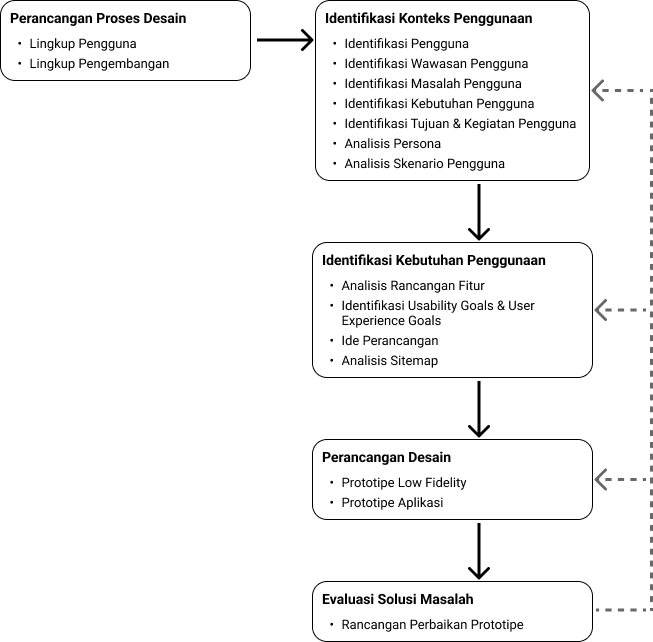
\includegraphics[width=0.8\textwidth]{chapter-3-alur-penelitian.png}
  \caption{Alur Kerja Penelitian}
  \label{fig:diagram_alur_kerja}
\end{figure}

\subsection{Perancangan Proses Desain}
Ruang lingkup yang ditentukan pada penelitian ini adalah sebagai berikut

\begin{enumerate}
  \item Lingkup Pengguna
  \subitem Target pengguna dari penelitian ini adalah masyarakat Indonesia yang pernah menggunakan atau memiliki ketertarikan terhadap aplikasi pencegah distraksi. Rentang usia dari target pengguna tidak dibatasi, namun difokuskan kepada golongan \textit{millenials} dengan rentang usia 18-30 tahun.
  \item Lingkup Pengembangan
  \subitem Desain interaksi aplikasi pencegah distraksi yang dibuat memiliki bentuk \textit{mobile interface} dengan mewujudkan sebuah prototipe aplikasi dalam \textit{platform Android}. Aplikasi Digital Wellbeing milik Google ditetapkan menjadi garis dasar pengembangan prototipe aplikasi tersebut.
\end{enumerate}


% \subsection{Identifikasi Konteks Penggunaan}

% Pada tahap ini dilakukan analisis hasil riset penggunaanalisis terhadap hasil riset yang


% \subsection{Identifikasi Kebutuhan Pengguna}


% \subsection{Perancangan Desain}


% \subsection{Evaluasi Solusi Masalah}



% % Ketiga solusi yang telah diuraikan pada subbab \ref{sec:analisis_solusi} akan diimplementasikan dalam prototipe aplikasi, beserta fitur-fitur lain pada Digital Wellbeing yang akan mendukung solusi tersebut. Prototipe aplikasi ini akan diimpementasikan pada \textit{platform} Android. Secara garis besar, proses perancangan prototipe aplikasi akan menggunakan pendekatan \textit{user-centered design} (UCD).

% Seperti yang telah disebutkan pada subbab \ref{sec:metodologi}, metodologi yang digunakan dalam pengerjaan Tugas Akhir ini akan menggunakan pendekatan UCD. Dengan maksud mengikuti prosesnya, maka langkah selanjutnya yang akan dilakukan adalah mengumpulkan data. Pengumpulan data akan dilakukan dengan menyebarkan form secara online serta melakukan wawancara dengan responden yang bersedia untuk bekerja sama lebih lanjut. Proses ini akan dilaksanakan pada periode pengerjaan Tugas Akhir 2. Pengumpulan data ini bertujuan untuk melakukan validasi terhadap permasalahan yang sudah dianalisis, dan juga tidak menutup kemungkinan untuk menemukan permasalahan desain interaksi lain dari masukan pengguna.

% Setelah melakukan pengumpulan data, akan dilakukan analisis terhadap masukan yang didapat untuk mejadi kebutuhan perangkat lunak. Hasil analisis juga akan memvalidasi analisis masalah dan solusi yang didapat dari observasi penulis pada subbab \ref{sec:analisis_masalah} dan \ref{sec:analisis_solusi}.

% Kebutuhan perangkat lunak yang telah disusun akan diimplementasi dalam bentuk prototipe \textit{low-fidelity} terlebih dahulu. Setelah dilakukan evaluasi, maka implementasi akan dilanjutkan dalam bentuk prototipe \textit{high-fidelity}. Setelah menjalani evaluasi, maka perancangan prototipe aplikasi akan dikerjakan. Prototipe aplikasi diharapkan akan menghasilkan data dengan kualitas yang lebih tinggi pada saat evaluasi dibandingkan saat menggunakan prototipe \textit{low-fidelity} atau \textit{high-fidelity}. Hasil evaluasi juga akan menentukan apakah aplikasi akan menjalani proses iterasi atau diimplementasi lebih lanjut.

% \blindtext